\documentclass[letterpaper,10pt]{examdesign}
\usepackage[utf8]{inputenc}
\usepackage{amsmath}
\usepackage{amsfonts}
\usepackage{amssymb}
\usepackage[spanish,es-noshorthands]{babel}
\usepackage[T1]{fontenc}
\usepackage{lmodern}
\usepackage{graphicx,hyperref}
\usepackage{tikz,pgf}
\usepackage{subfig}
\usepackage{wrapfig}
\usepackage[includeheadfoot,left=0.4in,right=0.4in,top=0.3in,bottom=0.2in]{geometry}
\NumberOfVersions{2}
\ShortKey
\class{
\includegraphics[height=1.7cm]{Images/logo-colegio.png} Matemáticas $9^{\circ}$}
\examname{Prueba bimestral I}
\def\namedata{\textbf{NO} marque ésta prueba. Conteste en el cuadro de respuestas y use una hoja en blanco para hacer sus operaciones}
\begin{document}
\begin{multiplechoice}[keycolumns=4,examcolumns=2]
\begin{block}[questions=2]
RESPONDE LAS 2 PREGUNTAS SIGUIENTES DE ACUERDO CON EL SIGUIENTE
GRÁFICO\\
\hspace*{1cm}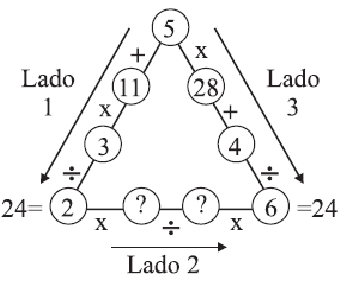
\includegraphics[scale=.55]{Images/triangulonum.png}
Sigue estrictamente el orden de las operaciones indicadas y verás que siempre llegas al mismo resultado.
\begin{question}
Los números que al ubicarse en el Lado 2 \textbf{NO} cumplen con la condición requerida para que el resultado final sea 24 son, respectivamente
\choice{4 y 2}
\choice{16 y 8}
\choice[!]{22 y 16}
\choice{26 y 13}
\end{question}
\begin{question}
Los números que aparecen dentro de los círculos del Lado 1, pertenecen al conjunto de los números
\choice{impares}
\choice[!]{primos}
\choice{pares}
\choice{enteros positivos}
\end{question}
\end{block}
\begin{block}[questions=2]
RESPONDE LAS DOS PREGUNTAS QUE SIGUEN DE ACUERDO CON LA SIGUIENTE INFORMACIÓN\\
De un tanque lleno de agua, con capacidad de 400 litros, se extrae 1/5  de agua el día lunes, 1/4 del agua restante el día martes y 9/30 del agua que queda en el tanque el día miércoles.
\begin{question}
La menor cantidad de agua se sacó el día
\choice{lunes}
\choice{martes}
\choice[!]{miércoles}
\choice{en los tres días se extrajo la misma cantidad de agua}
\end{question}
\begin{question}
¿Qué cantidad de agua queda disponible para el día jueves?
\choice{100 litros}
\choice[!]{168 litros}
\choice{175 litros}
\choice{232 litros}
\end{question}
\end{block}
\begin{question}
Si 48 de los 60 asientos en un autobús estaban ocupados, ¿qué porcentaje de los asientos NO estaba ocupado?
\choice{12\%}
\choice[!]{20\%}
\choice{25\%}
\choice{60\%}
\end{question}
\begin{question}
Un closet contiene 24 pares de zapatos. Si el 25\% de esos pares de zapatos son negros, ¿cuántos pares NO son negros?
\choice{4}
\choice{6}
\choice{12}
\choice[!]{18}
\end{question}
\begin{question}
¿Cuál de los siguientes es igual a $25(27+29+31)$?
\choice{$25(27+29)+31$}
\choice{25(27)+29+31}
\choice[!]{25(27)+(29+31)(25)}
\choice{25+(27)(29)(31)}
\end{question}
\begin{question}
¿Cuál de las siguientes fracciones NO es igual a $\dfrac{36}{45}$?
\choice{$\frac{4}{5}$}
\choice{$\frac{12}{15}$}
\choice[!]{$\frac{24}{35}$}
\choice{$\frac{48}{60}$}
\end{question}
\begin{question}
Al resolver $\dfrac{7}{5}\times \left(\dfrac{3}{7}-\dfrac{2}{5}\right)$, se obtiene
\choice{$\frac{1}{165}$}
\choice{$\frac{1}{35}$}
\choice[!]{$\frac{1}{25}$}
\choice{$\frac{19}{15}$}
\end{question}
\begin{question}
En la figura el \'angulo central es recto, ¿cuál es el valor de $x+y$?
\begin{center}
\begin{tikzpicture}[scale=.75]
\draw (-3,0)node[left]{$A$}--(3,0)node[right]{$D$};
\draw (-2,2)node[left]{$B$}--(0,0)--(2,2)node[right]{$C$};
\draw (-.25,.25)--(0,0.5)--(.25,.25);
\node[above left] at (-.25,0){$x$};
\node[above right]at (.25,0){$y$};
\end{tikzpicture}
\end{center}
\choice{30}
\choice{45}
\choice{110}
\choice[!]{90}
\end{question}
\begin{question}
Observa los siguientes triángulos; 
Sabiendo que los triángulos son semejantes y la medida de sus lados son proporcionales, entonces el valor de $a$ es:
\begin{center}
\begin{tikzpicture}[scale=.3]
\draw (0,0)--node[left]{$5\mu$}(0,5)--(15,0)--node[below]{$15\mu$}cycle;
\draw (17,0)--node[left]{$a$}(17,2)--(23,0)--cycle;
\node[below]at(20,0){$3\mu$};
\end{tikzpicture}
\end{center}
\choice[!]{1}
\choice{3}
\choice{5}
\choice{15}
\end{question}
\begin{question}
En la figura, ABCD es un cuadrado con centro en el origen. Si las coordenadas del vértice A son (4,4), ¿cuáles con las coordenadas del vértice C?
\begin{center}
\begin{tikzpicture}[scale=.35]
\draw[->] (-6,0)--(6,0)node[right]{$x$};
\draw[->] (0,-6)--(0,6)node[right]{$y$};
\draw (-4,-4)node[below]{$C$} rectangle (4,4)node[right]{$A(4,4)$};
\node[left] at (-4,4){$D$};
\node[right] (B) at (4,-4) {$B$};
\node[below left] at (0,0) {$O$};
\end{tikzpicture}
\end{center}
\choice{$(-4\sqrt{2},-4\sqrt{2})$}
\choice{$(-4\sqrt{2},-4)$}
\choice[!]{$(-4,-4)$}
\choice{$(-4,4)$}
\end{question}
\begin{block}[questions=2]
Un número se denomina perfecto cuando puede expresarse como la suma de sus divisores
positivos, excluyendo el número mismo.
\begin{question}
¿Cuál de los siguientes números es perfecto?
\choice{3}
\choice[!]{6}
\choice{10}
\choice{15}
\end{question}
\begin{question}
¿Es 28 un número perfecto?
\choice[!]{Sí, porque 28 = 1 + 2 + 4 + 7 + 14}
\choice{Sí, porque 28 = 2 + 5 + 7 + 14}
\choice{No, porque 28 es un número par.}
\choice{No, porque 28 tiene cuatro divisores.}
\end{question}
\end{block}
\begin{question}
La profesora de quinto de primaria les pidió a sus alumnos determinar el precio de una
caja de 6 huevos, sabiendo que cada uno vale \$250.\\
Cuatro estudiantes propusieron los siguientes procedimientos para encontrar la solución:
\begin{tabbing}
\hspace{1.5cm}\=\kill
Juan: \> $6\times 250$\\ 
Liliana: \> $6\times 25$ \\ 
Carlos: \> $250+6$\\ 
Milena \> $250+250+250+250+250+250$ 
\end{tabbing} 
¿Quiénes plantearon procedimientos correctos?
\choice[!]{Juan y Milena}
\choice{Liliana y Juan}
\choice{Juan y Carlos}
\choice{Milena y Liliana}
\end{question}
\begin{question}
Diego intent\'o solucionar la ecuación $x+3=5-x$, pero en uno de los pasos cometió un
error. Observa su solución:
\begin{align}
x+x&=5-3\\
2x&=2\\
x&=2-2\\
x&=0
\end{align}
¿En cuál de los pasos cometió el error?
\choice{En el paso 1}
\choice{En el paso 2}
\choice[!]{En el paso 3}
\choice{En el paso 4}
\end{question}
\begin{question}
La edad de un abuelo es el cuádruple de la edad de su nieto y la suma de sus edades es 90 años. Las edades del abuelo y su nieto en años respectivamente son:
\choice{80 y 10}
\choice{60 y 30}
\choice[!]{72 y 18}
\choice{75 y 15}
\end{question}
\begin{question}
El perímetro de un triángulo isósceles es 34 cm, siendo sus lados iguales 2 cm más que el tercer lado. Los lados del triángulo miden:
\choice{13, 13 y 11}
\choice{11, 14 y 9}
\choice{15, 15 y 13}
\choice[!]{12, 12 y 10}
\end{question}
\end{multiplechoice}
\end{document}